% Für Bindekorrektur als optionales Argument "BCORfaktormitmaßeinheit", dann
% sieht auch Option "twoside" vernünftig aus
% Näheres zu "scrartcl" bzw. "scrreprt" und "scrbook" siehe KOMA-Skript Doku
\documentclass[12pt,a4paper,titlepage,headinclude]{scrartcl}

%%%%%%%%%%%%%%%%%%%%%%%%%%%%%% Formatierung %%%%%%%%%%%%%%%%%%%%%%%%%%%

%keine Einrückung nach leerzeile
\parindent0pt

% Für Kopf und Fußzeilen, siehe auch KOMA-Skript Doku
\usepackage[komastyle]{scrpage2}
\pagestyle{scrheadings}
\setheadsepline{0.5pt}[\color{black}]
\automark[section]{chapter}

%Zitate und Literaturverzeichnis
\usepackage[backend=bibtex,natbib=true,sorting=nyt,style=numeric-comp]{biblatex}
\usepackage[babel,german=quotes]{csquotes}
\bibliography{literatur}

%Zur vernünftigen Dekodierung
\usepackage[T1]{fontenc} %
\usepackage[utf8]{inputenc} %utfx8
\usepackage[ngerman]{babel} %

%Interaktives Dokument
\usepackage[pdfpagelabels=true]{hyperref}%

%Für wissenschaftliches Zitieren
%\usepackage{natbib}

%Schriftarten
%\usepackage{lmodern} %

%Formatierung für Kof- und Fußzeile. Hier gilt entweder ... oder ...!!

%Für eigenen Zeilenabstand
\usepackage{setspace} %



%Für die Seitenformatierung
\usepackage{lscape} %
\usepackage{multicol} %
\usepackage{wallpaper} %

%Styling Inhaltsverzeichnis
\usepackage{tocloft} %

% Zur Formatierung für Kopf und Fußzeilen. Im Allgemeinen ist scrpage2 besser als fancyhdr
\usepackage{scrpage2}
\pagestyle{scrheadings}
\setheadsepline{0.5pt}[\color{black}]

%Einstellungen für Figuren- und Tabellenbeschriftungen
\setkomafont{captionlabel}{\sffamily\bfseries}
\setcapindent{0em} 


%%%%%%%%%%%%%%%%%%%%%%%%%%%%%% Mathematisches %%%%%%%%%%%%%%%%%%%%%%%%%%%

%Pakete für Mathesymbole
\usepackage{latexsym,exscale,stmaryrd} %
\usepackage{amssymb, amsfonts, amstext} %
\usepackage{amsmath, mathtools, amsthm} %

%Formelnummerierungen
\numberwithin{equation}{subsection}

% Weitere Symbole
\usepackage[nointegrals]{wasysym} %
\usepackage{eurosym} %
\usepackage{textcomp} %

%\usepackage{ucs} %

%Für vernünftige Einheiten 
\usepackage[separate-uncertainty, exponent-product = \cdot]{siunitx}
%\usepackage[thinspace,thinqspace,amssymb]{SIunits} %
\usepackage{icomma} %
\usepackage{nicefrac}%

%SI-Einheiten
\usepackage{siunitx}

%%%%%%%%%%%%%%%%%%%%%%%%%%%%%% Grafiken & Tabellen %%%%%%%%%%%%%%%%%%%%%%%%%%%
% Text umfließt Graphiken und Tabellen
% Beispiel:
% \begin{wrapfigure}[Zeilenanzahl]{"l" oder "r"}{breite}
%   \centering
%   \includegraphics[width=...]{grafik}
%   \caption{Beschriftung} 
%   \label{fig:grafik}
% \end{wrapfigure}
% Mehrere Abbildungen nebeneinander
% Beispiel:
% \begin{figure}[htb]
%   \centering
%   \subfigure[Beschriftung 1\label{fig:label1}]
%   {\includegraphics[width=0.49\textwidth]{grafik1}}
%   \hfill
%   \subfigure[Beschriftung 2\label{fig:label2}]
%   {\includegraphics[width=0.49\textwidth]{grafik2}}
%   \caption{Beschriftung allgemein}
%   \label{fig:label-gesamt}
% \end{figure}
% Caption neben Abbildung
% Beispiel:
% \sidecaptionvpos{figure}{"c" oder "t" oder "b"}
% \begin{SCfigure}[rel. Breite (normalerweise = 1)][hbt]
%   \centering
%   \includegraphics[width=0.5\textwidth]{grafik.png}
%   \caption{Beschreibung}
%   \label{fig:}
% \end{SCfigure}

%Einstellungen für Figuren- und Tabellenbeschriftungen
\setkomafont{captionlabel}{\sffamily\bfseries}
\setcapindent{0em}
\usepackage{transparent}%Für inkscape Grafiken

%Fuer mehr Platz in den Tabellen
\usepackage{cellspace} %mehr Platz in Tabellen
\addtolength\cellspacetoplimit{3pt}
\newcommand\myhline[1][2pt]{\\[#1]\hline}

%Zum Einbinden von GRafiken
\usepackage{graphicx}% [pdflatex]
\usepackage{xcolor}%

%Für textumflossene Grafiken
\usepackage{wrapfig} %

%Für subfigure
\usepackage{caption}
\usepackage{subcaption}

% Caption neben Abbildung
\usepackage{sidecap}

%Für URLs
\usepackage{url}%

%Zum Einbinden von Quelltext
\usepackage{listings-ext} %

%Für chemische Formeln
\usepackage{chemfig} %
%Für chemische Formeln (von www.dante.de)
%% Anpassung an LaTeX(2e) von Bernd Raichle
\makeatletter
\DeclareRobustCommand{\chemical}[1]{%
  {\(\m@th
   \edef\resetfontdimens{\noexpand\)%
       \fontdimen16\textfont2=\the\fontdimen16\textfont2
       \fontdimen17\textfont2=\the\fontdimen17\textfont2\relax}%
   \fontdimen16\textfont2=2.7pt \fontdimen17\textfont2=2.7pt
   \mathrm{#1}%
   \resetfontdimens}}
\makeatother
%erzwinge Fussnote auf selber Seite
\interfootnotelinepenalty=1000

%Zusätzliche Boxen
\usepackage{fancybox}

%\usepackage{framed}
%\usepackage{mathmode}
%\usepackage{empheq}

%Für variable Referenzen
\usepackage{varioref}

%Für Tabellen mit fester Gesamtbreite und variabler Spaltenbreite (im Gegensatz zu tabular)
\usepackage{tabularx}
%\newcommand{\ltab}{\raggedright\arraybackslash} % Tabellenabschnitt linksbündig
%\newcommand{\ctab}{\centering\arraybackslash} % Tabellenabschnitt zentriert
%\newcommand{\rtab}{\raggedleft\arraybackslash} % Tabellenabschnitt rechtsbündig


%Für Gleitobjekte
\usepackage{float} %Für H-Option

\usepackage{multirow} % Zellen von Tabellen zusammenfassen
\usepackage{booktabs} % verschoenert Tabellen
\usepackage{fixltx2e} % Repariert einige Dinge in Bezug auf das setzen von Gleitobjekten http://ctan.org/pkg/fixltx2e
\usepackage{stfloats} % Bei Gleitobjekten (figure,table,...) die ueber zwei Spalten gesetzt werden (Umgebung figure*), funktioniert [tb] http://ctan.org/pkg/stfloats
\usepackage{rotating} % Wird für Text und Grafiken benötigt, die um einen Winkel gedreht werden sollen



%%%%%%%%%%%%%%%%%%%%%%%%%%%%%% Kommandodefinitionen %%%%%%%%%%%%%%%%%%%%%%%%%%%

%Zur Korrektur und Kommentierung
\newcommand{\comment}[1]{\marginpar{\tiny{\textcolor{red}{#1}}}} % ermoeglicht kleine Kommentare am Seitenrand: \comment{Fehler?}
\newcommand{\Comment}[1]{\textcolor{red}{#1}}

%Zur Formatierung in der Matheumgebung
\renewcommand{\t}{\ensuremath{\rm\tiny}} % Tiefgestellter Text in der Matheumgebung wird schoener mit: $\Phi_{\t{Text}}$
\renewcommand{\d}{\ensuremath{\mathrm{d}}} % Die totale Ableitung ist stets aufrecht zu setzen: \d
\newcommand{\diff}[3][]{\ensuremath{\frac{\d^{#1}#2}{\d#3^{#1}}}} % einfache Ableitung nach x: $\ddx{\Phi}$
\newcommand{\pdiff}[3][]{\ensuremath{\frac{\partial^{#1}#2}{\partial#3^{#1}}}} % wie gesprochen, eine partielle Ableitung: \del
\newcommand{\aeqiv}{\ensuremath{\qquad \Longleftrightarrow \qquad}} % Eine Aequivalenz
\newcommand{\folgt}{\ensuremath{\qquad \Longrightarrow \qquad}} % Ein Folgepfeil mit Abstaenden
\newcommand{\corresponds}{\ensuremath{\mathrel{\widehat{=}}}} % Befehl für "Entspricht"-Zeichen
\newcommand{\mi}[1]{\ensuremath{\mathit{#1}}} % italics für griechische Buchstaben in Matheumgebung

%Um nicht so viel schreiben zu müssen...
\newcommand{\bs}[1]{\boldsymbol{#1}}
\newcommand{\ol}[1]{\overline{#1}}
\newcommand{\wtilde}[1]{\widetilde{#1}}
\newcommand{\mrm}[1]{\mathrm{#1}}
\newcommand{\mbf}[1]{\mathbf{#1}}
\newcommand{\mbb}[1]{\mathbb{#1}}
\newcommand{\mcal}[1]{\mathcal{#1}}
\newcommand{\mfrak}[1]{\mathfrak{#1}}

%Abkürzungen
\newcommand{\zB}{z.\,B.\ }
\newcommand{\bzw}{b.\,z.\, w.\ }
\newcommand{\Dh}{d.\,h.\ }
\newcommand{\Gl}{Gl.\ }
\newcommand{\Abb}{Abb.\ }
\newcommand{\Tab}{Tab.\ }

%Farbige Box um eine Formel
%Anwendung:
%\eqbox{
%  \begin{equation}
%    ...
%  \end{equation}
%}
\newcommand{\eqbox}[1]{
  \colorbox{gray!30}{\parbox{\linewidth}{#1}} 
}

%Im Text
\newcommand{\engl}[1]{engl. \textit{#1}}
\newcommand{\zitat}[1]{\footnote{#1}}
\newcommand{\person}[1]{\textsc{#1}}


%Matheoperatoren
\DeclareMathOperator{\tr}{tr}
\DeclareMathOperator{\sgn}{sgn}
\DeclareMathOperator{\diag}{diag}
\DeclareMathOperator{\const}{const}
\DeclareMathOperator{\grad}{grad}
\DeclareMathOperator{\rot}{rot}
\DeclareMathOperator{\divz}{div}


%%%%%%%%%%%%%%%%%%%%%%%%% Quellcode - Formatierung %%%%%%%%%%%%%%%%%%%%%%%%%%%%%%%%%%%%%%

%Um auch Umlaute in den Kommentaren auswerten zu können
\lstset{
literate = {Ö}{{\"O}}1 {Ä}{{\"A}}1 {Ü}{{\"U}}1 {ß}{{\ss}}2 {ü}{{\"u}}1
           {ä}{{\"a}}1 {ö}{{\"o}}1
}

%Formatierung des Quellcode
\lstset{
language=C++,
basicstyle=\footnotesize\ttfamily,
keywordstyle=\bfseries\color{blue},
stringstyle=\color{red},
commentstyle=\itshape\color{green!60!black},
emphstyle = \bfseries\color{red!80!green!60!blue}
%identifierstyle=,
}

%Zum Hervorheben bestimmter Begriffe (z.B. eigene Klassen, etc.)
%\lstset{
%emph = {vector, iterator, std, ostream, istream , ofstream, ifstream, fstream, cmath}
%}

%Nummerirung
\lstset{
numbers=left,
numberstyle=\tiny,
stepnumber=2,
numbersep=5pt,
frame=single,
breaklines=true
framesep=5pt,
numbersep=8pt,
breakindent=3ex
}

%Einbunden über
%\lstinputlisting[caption={blablabla}, language=C++]{name.cpp}

\begin{document}
%Autor, etc.
\newcommand{\versuch}{Versuch 14}
\newcommand{\titel}{Wechselstromwiderstände}
\newcommand{\praktikantA}{Eric Bertok}
\newcommand{\praktikantB}{Kevin Lüdemann}
\newcommand{\betreuer}{Björn Klaas}
\newcommand{\emailA}{
      \href{mailto:eric.bertok@stud.uni-goettingen.de }
           {eric.bertok@stud.uni-goettingen.de} }
\newcommand{\emailB}{
      \href{kevin.luedemann@stud.uni-goettingen.de}
           {kevin.luedemann@stud.uni-goettingen.de} }
\newcommand{\gruppe}{B002}
\newcommand{\durchfuehrungsdatum}{08.09.2014}
\newcommand{\abgabedatum}{05.10.2014}

%Metainformationen
\hypersetup{
      pdfauthor = {\praktikantA~ },
      pdftitle  = {\versuch: \titel},
      pdfsubject = {\titel}
}

\begin{titlepage}
\centering
\textsc{\Large Anfängerpraktikum der Fakultät für
  Physik,\\[1.5ex] Universität Göttingen}

\vspace*{2.5cm}

\rule{\textwidth}{1pt}\\[0.5cm]
{\huge \bfseries
  \versuch\\[1.5ex]
  \titel}\\[0.5cm]
\rule{\textwidth}{1pt}

\vspace*{2.5cm}

\begin{Large}
\begin{tabular}{ll}
Praktikant: &  \praktikantA\\
Mitarbeiter:	      &  \praktikantB \\
Email:	& \emailA\\
	& \emailB\\
Gruppe: & \gruppe\\
Betreuer: & \betreuer\\
Durchgeführt am: & \durchfuehrungsdatum\\
Abgegeben am: & \abgabedatum\\
\end{tabular}
\end{Large}
\vspace*{0.8cm}

\begin{Large}
\fbox{
  \begin{minipage}[t][2.5cm][t]{6cm} 
    Testat:
  \end{minipage}
}
\end{Large}

\end{titlepage}

\cleardoublepage
\tableofcontents
\thispagestyle{empty}
\cleardoublepage

\setcounter{footnote}{0}
\setcounter{page}{1}

\pagenumbering{arabic}

\newpage

\section{Einleitung}
\label{sec:einleitung}
Der Wechselstrom hat sich in vielen Bereichen der Technik gegenüber dem Gleichstrom durchgesetzt. Zum einen ist er durch Generatoren leichter zu erzeugen, zum anderen ist eine einfache Transformation der Spannung möglich (siehe Versuch 16 - "Der Transformator"). In diesem Versuch wird das Verhalten von Spule, Kondensator und dem \person{Ohm}schen Widerstand bei Wechselspannung untersucht. Durch Messung der Phasenverschiebung zwischen Strom und Spannung und deren Größenverhältnisse wird die Theorie der komplexen Wechselstromwiderstände getestet.
\section{Theorie}
\subsection{Wechselstrom}
\label{sec:theorie}
Betrachtet wird ein Stromkreis, an dem eine äußere periodische Wechselspannung der Form
\begin{align}
	U_e(t)=U_0\cdot\cos(\omega t)
	\label{eq:wechselspannung}
\end{align}
anliegt. Dabei ist $U_0$ die Scheitelspannung und $\omega=\frac{2\pi}{T}$ die Kreisfrequenz. Im Allgemeinen besitzt der hieraus entstehende Wechselstrom zusätzlich zu seiner Amplitude $I_0$ eine Phasenverschiebung $\varphi$. So lässt sich der Strom $I$ als
\begin{align}
	I(t)=I_0\cdot\cos(\omega t-\varphi)
	\label{eq:wechselstrom}
\end{align}
schreiben. Es ist üblich, zur Vereinfachung Strom und Spannung als komplexe Größen zu schreiben \cite[253]{nol3}:
\begin{align}
	U_e(t)&=U_0e^{i\omega t}
	\label{eq:complexspannung}\\
	I(t)&=I_0e^{i(\omega t-\varphi)}.
	\label{eq:complexstrom}
\end{align}
Dabei ist der Realteil stets der physikalisch relevante Wert.
Als Verallgemeinerung des Widerstands wird der komplexe Widerstand $Z$ eingeführt \cite[254]{nol3}:
\begin{align}
	Z=\frac{U_e}{I}=\frac{U_0}{I_0}e^{i\varphi}.
	\label{eq:z}
\end{align}
\subsection{\person{Ohm}scher Widerstand}
Betrachtet man einen Stromkreis, welcher nur aus einem \person{Ohm}schen Widerstand besteht, so gilt nach dem \person{Ohm}schen Gesetz
\begin{align}
	U(t)=R\cdot I,
	\label{eq:ohm}
\end{align}
dass der Strom keine Phasenverschiebung zur Spannung aufweist. Somit ist $Z$ reell:
\begin{align}
	Z_{R}=\operatorname{Re}(Z)=R.
	\label{eq:zR}
\end{align}
\subsection{Induktiver Widerstand}
Nun besteht der Stromkreis aus einer reinen Induktivität $L$. Zum einen folgt aus der \person{Kirchhoff}schen Maschenregel \cite[55]{demtroeder2}
\begin{align}
	U_e+U_{ind}=0,
	\label{eq:indmasche}
\end{align}
zum anderen gilt nach dem Induktionsgesetz \cite[131]{demtroeder2}:
\begin{align}
	U_{ind}=-L\cdot\frac{\d I}{\d t}.
	\label{eq:uind}
\end{align}
Durch Einsetzen und Integration erhält man als induktiven Widerstand \cite[256]{nol3}
\begin{align}
	Z_{L}=i\omega L,
	\label{eq:zL}
\end{align}
welcher rein imaginär ist. Der Strom ist um $\varphi=\frac{\pi}{2}$ gegenüber der Spannung verzögert.
\subsection{Kapazitiver Widerstand}
Jetzt besteht der Stromkreis, an dem die Wechselspannung anliegt, lediglich aus einer Kapazität $C$. Für die Spannung an einem Kondensator gilt \cite[152]{demtroeder2}
\begin{align}
	U_e=\frac{Q}{C}.
	\label{eq:kond}
\end{align}
Durch Differentiation erhält man \cite[257]{nol3}:
\begin{align}
	I(t)&=\frac{\d U_e}{\d t}C=i\omega C~ U_e\\
	\aeqiv U_e(t)&=\frac{1}{i\omega C}I(t)=-\frac{i}{\omega C}I(t).
	\label{eq:herleitungzC}
\end{align}
Für den kapazitiven Widerstand $Z_C$ ergibt sich also:
\begin{align}
	Z_C=-\frac{i}{\omega C}.
	\label{eq:zC}
\end{align}
Der Strom eilt der Spannung um $\frac{\pi}{2}$ voraus, $\varphi=-\frac{\pi}{2}$.
\subsection{Reihen- und Parallelschaltung von komplexen Widerständen}
\label{sec:reihepara}
Die Reihen- und Parallelschaltung von komplexen Widerständen geht analog zu normalen Widerständen. Bei einer Reihenschaltung fließt durch alle Bauteile der gleiche Strom und die Spannungen werden addiert. Folglich werden auch die komplexen Widerstände addiert. Für einen Serienkreis mit \person{Ohm}schen Widerstand, Induktivität und Kapazität gilt:
\begin{align}
	Z=Z_R+Z_L+Z_C=R+i\left( \omega L-\frac{1}{\omega C} \right).
	\label{eq:zserie}
\end{align}
Bei einer Parallelschaltung ist die an jedem Bauteil anliegende Spannung identisch. Nach der Knotenregel \cite[55]{demtroeder2} addieren sich die Ströme:
\begin{align}
	\frac{U_e}{Z}=I=I_R+I_L+I_C&=\frac{U_e}{Z_R}+\frac{U_e}{Z_L}+\frac{U_e}{Z_C}\\
	\aeqiv \frac{1}{Z}&=\frac{1}{Z_R}+\frac{1}{Z_L}+\frac{1}{Z_C}\\
	&=\frac{1}{R}+i\left( \omega C- \frac{1}{\omega L}\right).
	\label{eq:zpara}
\end{align}
\subsection{Beträge und Phasenverschiebungen}
Die obigen Ergebnisse lassen sich sehr anschaulich in der komplexen Zahlenebene darstellen. In Abbildung \ref{fig:theozeiger} ist das Ergebnis aus Gleichung \eqref{eq:zserie} veranschaulicht. 
\begin{figure}[htb]
	\centering
	\input{zeiger.pdf_tex}
	\caption{Darstellung des komplexen Widerstandes $Z$ in der komplexen Ebene.}
	\label{fig:theozeiger}
\end{figure}
Durch den Quotienten von Imaginär- und Realteil lässt sich ein Ausdruck für die Phasenverschiebung $\varphi$ angeben \cite[153]{demtroeder2}:
\begin{align}
	\tan\varphi=\frac{\operatorname{Im}(Z)}{\operatorname{Re}(Z)}=\frac{\omega L-\frac{1}{\omega C}}{R}.
	\label{eq:phase}
\end{align}
Den Betrag vom komplexen Widerstand 
\begin{align}
	|Z|=\sqrt{\operatorname{Re}(Z)^2+\operatorname{Im}(Z)^2}=\sqrt{R^2+\left(\omega L-\frac{1}{\omega C}\right)^2}
	\label{eq:impedanz}
\end{align}
bezeichnet man als Impedanz.
\section{Durchführung}
\label{sec:durchfuehrung}

\subsection{Versuchsaufbau und benötigte Materialien}
\begin{figure}[h!]
	\centering
	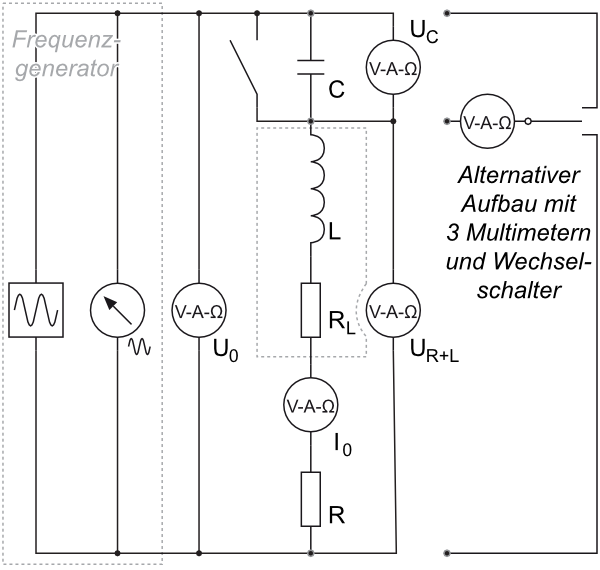
\includegraphics{reihe.png}
	\caption{Schaltskizze für den Serienkreis \cite[Abgerufen am: 05.10.2014]{LP14}}
	\label{fig:schaltreihe}
\end{figure}
\begin{figure}[h!]
	\centering
	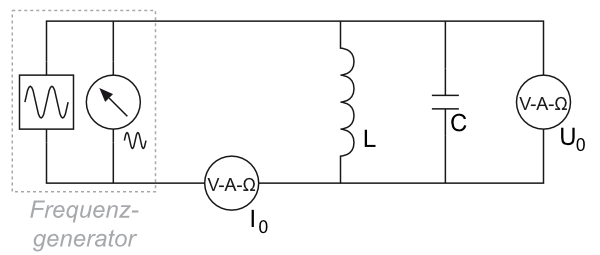
\includegraphics{para.png}
	\caption{Schaltskizze für den Parallelkreis \cite[Abgerufen am: 05.10.2014]{LP14}}
	\label{fig:schaltpara}
\end{figure}

In den Abbildungen \ref{fig:schaltreihe} und \ref{fig:schaltpara} sind die Schaltskizzen der beiden Versuchsaufbauten zu sehen. Benötigt werden eine Wechselspannungsquelle mit variabler Frequenz, ein Kondensator, eine Luftspule, ein \person{Ohm}scher Widerstand, ein Schalter, ein Digitaloszilloskop und vier Multimeter. 
\subsection{Serienkreis ohne Kondensator}
\label{sec:serie1}
Für den ersten Versuchsteil werden die Bauteile gemäß Abbildungen \ref{fig:schaltreihe} und \ref{fig:schaltpara} in Reihe geschaltet. Der Schalter wird geöffnet, um den Kondensator zu überbrücken. Durch das Oszilloskop darf kein Strom fließen. Um die Phasenverschiebung zwischen Strom und Spannung zu messen, wird es deswegen sowohl direkt an die Spannungsquelle als auch parallel zum \person{Ohm}schen Widerstand geschaltet. Nun wird in einem Frequenzbereich von ca. 60 bis 480\;Hz für zehn verschiedene Frequenzen der Strom $I$ durch den \person{Ohm}schen Widerstand, die Gesamtspannung $U$ und die Phasenverschiebung  $\varphi$ zwischen Strom und Spannung gemessen. Die Spannung kann dabei an der Spannungsquelle eingestellt werden. Gemessen wird sie trotz der Anzeige der Spannungsquelle am Oszilloskop, da sie dort genauer ausgegeben wird. Die Phasenverschiebung ist ebenfalls am Oszilloskop abzulesen. Dafür muss sich dieses in dem Modus "`Messung"' befinden. Zu beachten ist, dass der Innenwiderstand des Amperemeters von dem eingestellten Messbereich abhängt. Um einer möglichen Verfälschung der Messwerte vorzubeugen, sollte deshalb für jeden Versuchsabschnitt ein einheitlicher Messbereich eingestellt werden. Die Widerstände der Voltmeter hingegen sind als unendlich angenommen.

\subsection{Serienkreis mit Kondensator}
Für diesen Versuchsteil wird der Schalter geöffnet, wodurch die Schaltung zu einem Serienschwingkreis wird. Wie in Sektion \ref{sec:serie1} wird für den gleichen Frequenzbereich die Gesamtspannung $U$, der Gesamtstrom $I$ und die Phasenverschiebung $\varphi$ gemessen. Hierbei ist darauf zu achten, die Resonanzstelle besonders genau abzutasten, um eine genaue Bestimmung der Resonanzfrequenz zu ermöglichen.

\subsection{Parallelkreis}
Nun wird der Parallelkreis ohne den \person{Ohm}schen Widerstand aus Abbildung \ref{fig:schaltpara} aufgebaut. Er besteht aus einer Spule  und einem parallel geschalteten Kondensator. Der in der Spule integrierte Spulenwiderstand $R_L$ ist in Reihe zu dieser geschaltet. Das Volt- und Amperemeter wird analog zu den vorherigen Schaltungen angeschlossen. Erneut wird die Spannung $U$, der Strom $I$ und die Phasenverschiebung $\varphi$ notiert, wobei die Resonanzstelle besonders genau vermessen wird.
\subsection{Ausmessung der Bauteile}
Als letztes werden mit den Multimetern die elektrischen Bauteile vermessen. Hierzu gehören der Innenwiderstand des Amperemeters für alle verwendeten Messbereiche, der Widerstand des \person{Ohm}schen Widerstandes, der Widerstand der Spule, sowie die Kapazität des Kondensators. Ebenfalls zu notieren sind der Durchmesser und die Windungszahl der Luftspule.
\section{Auswertung}
\label{sec:auswertung}
\subsection{Bestimmung der Induktivität und des \person{Ohm}schen Widerstands beim Serienkreis ohne Kondensator}
\label{sec:lin}
Aus der Messreihe für den Serienkreis bei überbrücktem Kondensator (Sektion \ref{sec:serie1}) sollen die Induktivität $L$ der Spule, sowie der gesamte \person{Ohm}sche Widerstand $R$, bestehend aus Spulenwiderstand $R_L$ und einzelnem \person{Ohm}schen Widerstand $R_\Omega$, bestimmt werden. Hierfür betrachtet man Gleichung \eqref{eq:zserie}. Da der Kondensator überbrückt ist, besteht der Imaginärteil, woraus für den komplexen Widerstand $Z$ gilt:
\begin{align}
	Z(\omega)=R+i~\omega L.
	\label{eq:impedRL}
\end{align}
Berechnet man nun die Impedanz gemäß Gleichung \eqref{eq:impedanz} und quadriert, so erhält man
\begin{align}
	\left( \frac{U}{I} \right)^2=Z_0^2=\underbrace{R^2}_b+\omega^2 \underbrace{L^2}_m.
	\label{eq:gerade}
\end{align}
Man erwartet also einen linearen Zusammenhang zwischen dem Impedanzquadrat $Z^2$ und dem Quadrat der Kreisfrequenz $\omega^2$. Die Steigung $m$ entspricht dabei dem Quadrat der Induktivität $L^2$ und der Ordinatenabschnitt wird als Quadrat des \person{Ohm}schen Gesamtwiderstands $R^2$ identifiziert.
Für die Messfehler der Multimeter wurde der größtmögliche Fehler nach \cite[35]{prakti} verwendet, da die während des Versuchs angenommenen Fehler zu klein sind. Sie sind In Tabelle \ref{tab:messfehler} zu sehen.
\begin{table}
	\centering
	\begin{tabular}{l|l}
		\hline
		Messbereich&Fehler\\\hline
		alle Spannungen&$1\%$ v. Messwert + 3 Digits\\
		alle Ströme&$1.5\%$ v Messwert + 3 Digits\\\hline
	\end{tabular}
	\caption{Messfehler der Multimeter}
	\label{tab:messfehler}
\end{table}
Der Fehler der Frequenz wurde einheitlich auf $\sigma_f=1$ gesetzt, da der auf dem Oszilloskop ausgegebene Wert innerhalb dieses Bereichs schwankte. Das Kreisfrequenzquadrat berechnet sich nach $\omega^2=\left( 2\pi f \right)^2$. Mit der \person{Gauss}schen Fehlerfortpflanzung ergibt sich ein Fehler von 
\begin{align}
	\sigma_{\omega^2}=8  \pi^{2}  f\cdot \sigma_{f}.
	\label{eq:sigmaomega}
\end{align}
 Der Fehler der gesamten Impedanz berechnet sich nach
\begin{align}
	\sigma_{Z_0^2}=\frac{2}{I^{3}} \cdot U \cdot \sqrt{I^{2} \cdot \sigma_{U}^{2} + U^{2} \cdot \sigma_{I}^{2}}.
	\label{eq:sigmaz0}
\end{align}
\begin{figure}[h!]
	\centering
	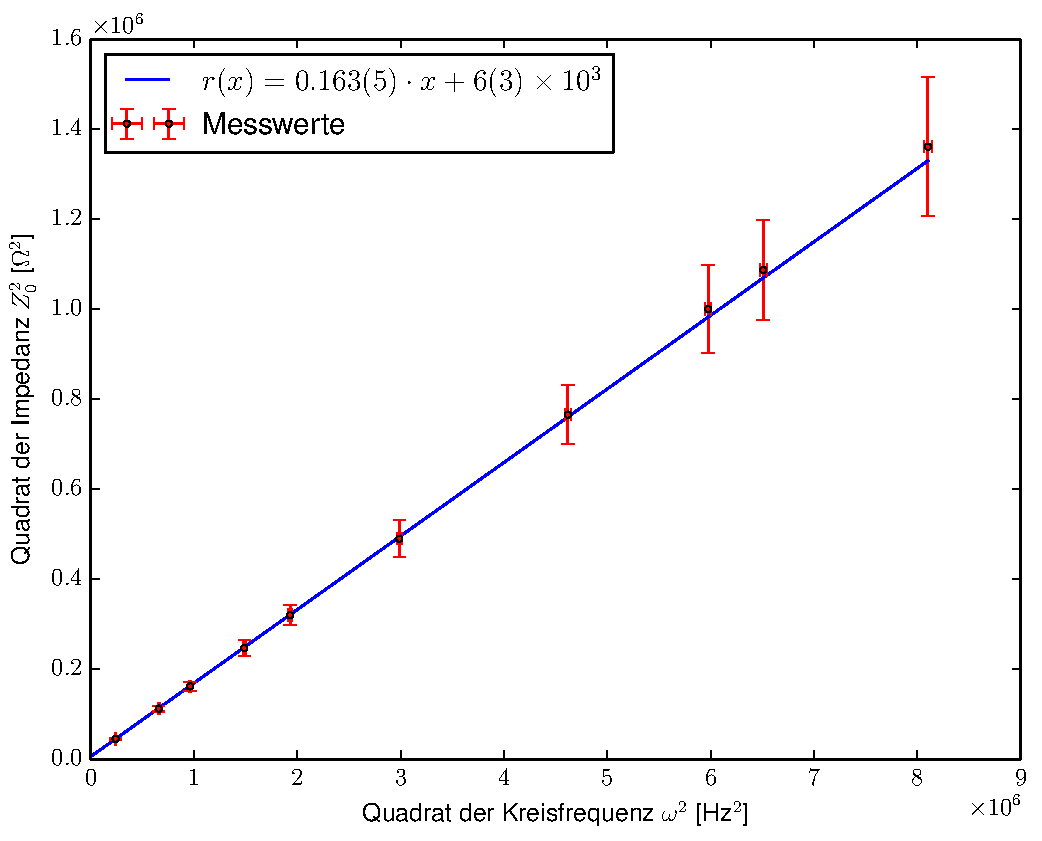
\includegraphics[width=\textwidth]{plot1.pdf}
	\caption{Auswertung des Serienkreises ohne Kondensator. Das Quadrat der Impedanz wird über dem Quadrat der Kreisfrequenz aufgetragen. Es ergibt sich wie erwartet ein linearer Zusammenhang. In rot sind die Messwerte samt Fehler, in blau die Regressionsgerade aufgetragen.}
	\label{fig:plot1}
\end{figure}
Die Auftragung des Impedanzquadrates über dem Kreisfrequenzquadrat ist in Abbildung \ref{fig:plot1} zu sehen. Anschließend wird eine lineare Regression durchgeführt. Die Regressionsgerade ist ebenfalls in Abbildung \ref{fig:plot1} eingezeichnet. Man erhält als Parameter:
\begin{align}
	m&=L^2=(0.163\pm0.005)~\mrm{H}^2\\
	b&=R^2=(6\pm3)\times 10^3~\mrm{\Omega}^2.
	\label{eq:plot1}
\end{align}
Nach \person{Gauss} ergibt sich für die Fehler von Induktivität $L$ und Widerstand $R$:
\begin{align}
	\sigma_L=\frac{1}{2\sqrt{m}}\cdot\sigma_m,\qquad\sigma_R=\frac{1}{2\sqrt{m}}\cdot\sigma_b.
	\label{eq:sigma1}
\end{align}
Es ergeben sich als Resultate:
\begin{align}
	L_{\mrm{lin}}&=(0.404\pm0.007)~\mrm{H}\\
	R_{\mrm{lin}}&=(76\pm18)~\mrm{\Omega}.
	\label{eq:result1}
\end{align}
\newpage
\subsection{Bestimmung der Resonanzfrequenz und des \person{Ohm}schen Widerstands beim Serienresonanzkreis}
\label{sec:serienresonanzkreis}
\begin{figure}[h!]
	\centering
	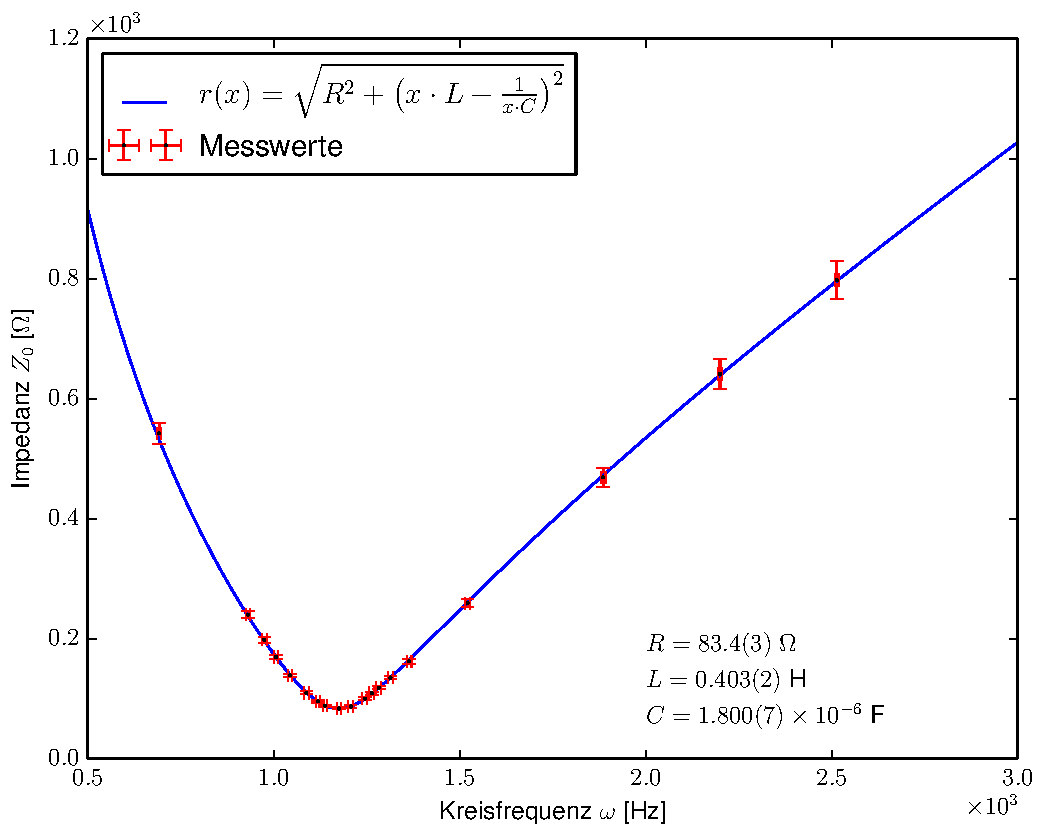
\includegraphics[width=\textwidth]{plot2.pdf}
	\caption{Auftragung der gesamten Impedanz $Z_0$ über der Kreisfrequenz $\omega$. In rot sind die Messwerte samt Fehler aufgetragen. Um die Parameter $R$, $L$ und $C$ zu bestimmen, wird ein nichtlinearer Fit durchgeführt. Die ermittelten Werte sind mit der Regressionskurve eingezeichnet.}
	\label{fig:plot2}
\end{figure}
Für diesen Auswertungsteil wird die gesamte Impedanz $Z_0=\frac{U}{I}$ über der Kreisfrequenz $\omega=2\pi\cdot f$ aufgetragen (Abbildung \ref{fig:plot2}). Die Messfehler werden analog zum ersten Auswertungsteil gewählt. Mit der \person{Gauss}schen Fehlerfortpflanzung berechnen sich die Fehler nach:
\begin{align}
	\sigma_{\omega}&=2 \cdot \pi \cdot \sigma_{f}\\
	\sigma_{Z_0}&=\frac{1}{I^{2}} \cdot \sqrt{I^{2} \cdot \sigma_{U}^{2} + U^{2} \cdot \sigma_{I}^{2}}.
	\label{eq:sigmaomegaz02}
\end{align}
Nach Gleichung \eqref{eq:impedanz} ist die Impedanz minimal, wenn $\omega L =\frac{1}{\omega C}$ gilt. Für die Resonanzfrequenz ergibt sich also
\begin{align}
	\omega_r=\sqrt{\frac{1}{LC}}.
	\label{eq:resonanz}
\end{align}
Beim Resonanzminumum gilt ferner $Z_0=R$. Mithilfe eines Python-Skriptes wird eine nichtlineare Regression nach Gleichung \eqref{eq:impedanz} durchgeführt und nach den Parametern $R$, $L$ und $C$ gefittet. Die Regression ergibt:
\begin{align}
	R_{\mrm{fit},1}&=(83.4\pm0.9)~\mrm{\Omega}
	\label{eq:Rfit1}\\
	L_{\mrm{fit},1}&=(0.403\pm0.005)~\mrm{H}
	\label{eq:Lfit1}\\
	C_{\mrm{fit},1}&=(1.80\pm0.02)~\SI{}{\micro\farad}.
	\label{eq:Cfit1}
\end{align}
Die Resonanzfrequenz wird nach Gleichung \eqref{eq:resonanz} berechnet. Man erhält
\begin{align}
	\sigma_{\omega_{r,1}}&=\sqrt{\frac{\sigma_L^2}{4\cdot L^3\cdot C}+\frac{\sigma_C^2}{4\cdot L\cdot C^3}}
	\label{eq:sigmaresonanzfrequenz1}\\
	\omega_{r,1}&=(1174 \pm 3)~\mrm{Hz}.\label{eq:resonanzfrequenz1}
\end{align}
\subsection{Bestimmung der Resonanzfrequenz aus der Phasenverschiebung}
\label{sec:phasenverschiebung}
\begin{figure}[H]
	\centering
	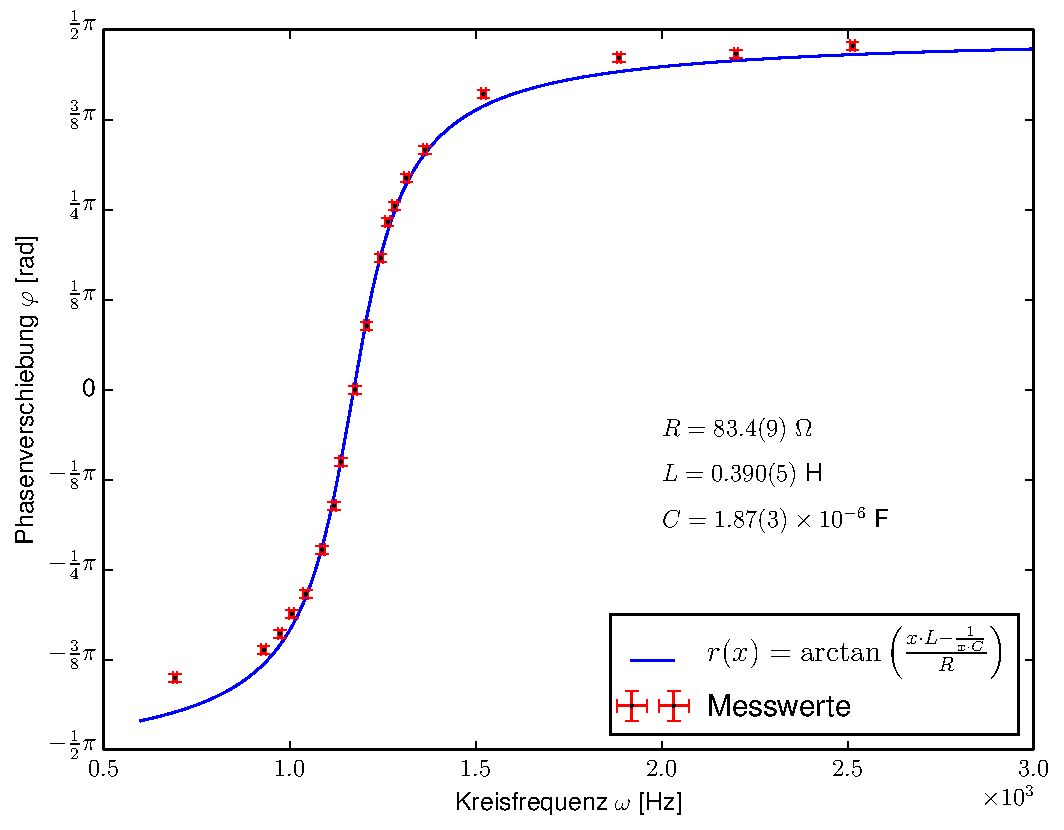
\includegraphics[width=0.85\textwidth]{plot3.pdf}
	\caption{Auftragung der Phasenverschiebung $\varphi$ zwischen Strom und Spannung über der Kreisfrequenz $\omega$. Die Resonanzfrequenz $\omega_r$ kann als Nullstelle direkt abgelesen werden. Weiterhin wird ein nichtlinearer Fit durchgeführt, wobei der \person{Ohm}sche Gesamtwiderstand $R$ konstant gehalten wird.}
	\label{fig:plot3}
\end{figure}
Mithilfe der Phasenverschiebung $\varphi$ soll erneut die Resonanzfrequenz $\omega_r$ ermittelt werden. Nach Gleichung \eqref{eq:phase} gilt bei der Resonanzfrequenz $\omega_r=\sqrt{\frac{1}{L\cdot C}}$:
	\begin{align}
		\varphi(\omega_r)=0.
		\label{eq:phaseresonanz}
	\end{align}
Normalerweise werden die Messwerte nahe der Nullstelle durch eine lineare Funktion interpoliert, um die exakte Resonanzfrequenz zu bestimmen. Bei der hier aufgenommenen Messreihe ist die Bestimmung jedoch trivial, da während des Versuchs bereits eine Phasenverschiebung von 0 gemessen wurde. Der Wert der Frequenz an dieser Stelle beträgt $f_r=(187\pm1)~$Hz. Es ergibt sich nach $\omega=2\pi\cdot f$ und der Fehlergleichung $\sigma_{\omega}=2 \cdot \pi \cdot \sigma_{f}$ für die Resonanzfrequenz:
\begin{align}
	\omega_{r,2}=(1175\pm7)~\mrm{Hz}.
	\label{eq:resonnanzfrequenz2}
\end{align}
Zusätzlich wird ein nichtlinearer Fit nach Gleichung \eqref{eq:phase} durchgeführt. Hierbei wird der \person{Ohm}sche Gesamtwiderstand $R$ auf den zuvor erhaltenen Wert dieser Messreihe aus der Regression in Sektion \ref{sec:serienresonanzkreis} $R_{\mrm{fit},1}=(83.4\pm0.09)~\mrm{\Omega}$ gesetzt. Wird dies nicht getan, so konvergiert der Fit nicht. Die Ergebnisse sind zusammen mit den Messwerten in Abbildung \ref{fig:plot3} zu sehen. Man erhält aus dem Fit:
\begin{align}
	L_{\mrm{fit},2}&=(0.390\pm0.005)~\mrm{H}
	\label{eq:Lfit2}\\
	C_{\mrm{fit},2}&=(1.87\pm0.03)~\SI{}{\micro\farad}.
	\label{eq:Cfit2}
\end{align}
\subsection{Bestimmung der Phasenverschiebung zwischen $U_{L+R}$ und $U_C$ aus dem Zeigerdiagramm}
\label{sec:zeiger}
Zunächst werden die Spannung am Kondensator $U_C$, die Spannung an Spule und \person{Ohm}schen Widerstand $U_{L+R}$ und die Gesamtspannung $U$ in Abhängigkeit von der Kreisfrequenz $\omega$ in ein gemeinsames Diagramm gezeichnet. Das Ergebnis ist in Abbildung \ref{fig:plot4} zu sehen. Man erkennt, dass $R$ in guter Näherung konstant ist. $U_{L+R}$ und $U_C$ haben ein deutliches Maximum an der Resonanzfrequenz. Es ist auch zu erkennen, dass unterhalb der Resonanzfrequenz $U_C$ größer als $U_{L+R}$ ist, während es oberhalb der Resonanzstelle umgekehrt ist. Dies zeigt, dass sich der Serienschwingkreis bei niedrigen Frequenzen hauptsächlich kapazitiv verhält und eher durch den Kondensator beschränkt ist, während bei hohen Frequenzen das Verhalten induktiv ist und hier die Spule blockiert. Die Spannungen während der Resonanz können wieder direkt abgelesen werden:
\begin{align}
	U_{L+R}=(54.6\pm0.6)~\mrm V,\qquad U_{C}=(53.5\pm0.6)~\mrm V.
	\label{eq:spannungen}
\end{align}
\begin{figure}[h!]
	\centering
	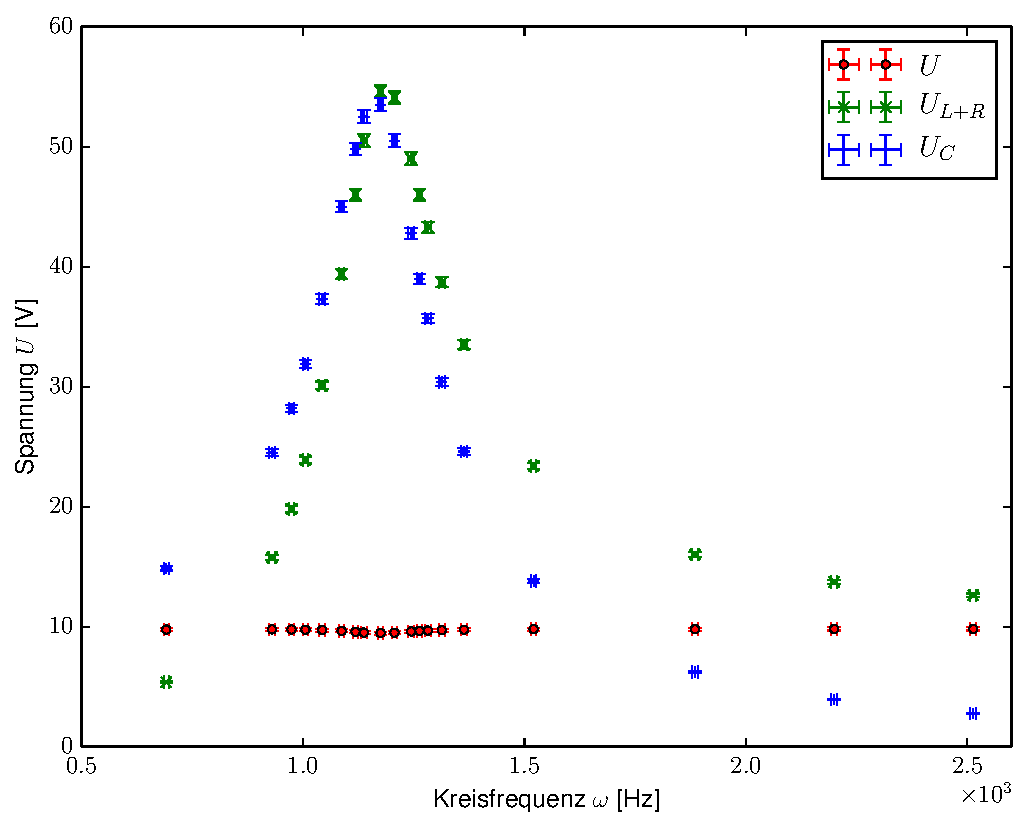
\includegraphics[width=0.85\textwidth]{plot4.pdf}
	\caption{Auftragung von der Gesamtspannung $U$, der Spannung an der Spule und dem \person{Ohm}schen Widerstand $U_{L+R}$ und der Spannung am Kondensator $U_C$ über der Kreisfrequenz $\omega.$} \label{fig:plot4}
\end{figure}
Der Zusammenhang zwischen diesen Größen wird in Abbildung \ref{fig:zeiger2} anhand eines Zeigerdiagramms  dargestellt.

\begin{figure}[h!]
	\centering
	\resizebox{4cm}{!}{\input{zeiger2.pdf_tex}}
	\caption{Zeigerdiagramm der gemessenen Spannungen.}
	\label{fig:zeiger2}
\end{figure}
Da die Resonanzfrequenz gezeigt ist, sind $U_L$ und $U_C$ gleich lang und entgegengesetzt. Es ist somit abzulesen:
\begin{align}
	\sin(\varphi)&=\frac{U_L}{U_{L+R}}=\frac{U_C}{U_{L+R}}\\
	\aeqiv\varphi&=\arcsin\left(\frac{U_C}{U_{L+R}}\right).
\end{align}
Mit der \person{Gauss}schen Fehlerfortpflanzung errechnet sich der Fehler nach
\begin{align}
	\sigma_{\varphi}=\frac{1}{U_{L+R}} \cdot \sqrt{\frac{1}{U_{C}^{2} - U_{L+R}^{2}} \cdot \left(- U_{C}^{2} \cdot \sigma_{U_{L+R}}^{2} - U_{L+R}^{2} \cdot \sigma_{U_{C}}^{2}\right)}.
	\label{eq:sigmaphasezeiger}
\end{align}
Es ergibt sich daraus eine Phasenverschiebung von
\begin{align}
	\varphi_{\text{Zeiger}}=(1.37\pm0.08)~\mrm{rad}.
	\label{eq:phasezeiger}
\end{align}
\subsection{Auswertung des Parallelschwingkreises}
\label{sec:parakreis}
Der verwendete Parallelschwingkreis besteht aus einem Kondensator, welcher parallel zu einer Reihenschaltung von der Spule und ihrem integrierten Spulenwiderstand geschaltet ist.
Nach den Regeln aus Sektion \ref{sec:reihepara} gilt:
\begin{align}
	\frac{1}{Z}=\frac{1}{R+i~\omega L}-\frac{1}{\frac{i}{\omega C}}.
	\label{eq:zpara}
\end{align}
Für die Impedanz ergibt sich nach Bildung des Betrags:
\begin{align}
	Z_0=\frac{R^2+\omega^2 L^2}{\sqrt{R^2+\left[ \omega C(R^2+\omega^2L^2)-\omega L \right]^2}}.
	\label{eq:impedpara}
\end{align}
Es werden analog zum Serienresonanzkreis die Werte der gesamten Impedanz $Z_0$ über der Kreisfrequenz $\omega$ aufgetragen. Mit Gleichung \eqref{eq:impedpara} wird ein nichtlinearer Fit durchgeführt. Das Ergebnis ist in Abbildung \ref{fig:plot5} zu sehen.
Die Ergebnisse des Fits sind:

\begin{align}
	R_{\mrm{fit},3}&=(70\pm3)~\mrm{\Omega}
	\label{eq:Rfit3}\\
	L_{\mrm{fit},3}&=(0.385\pm0.005)~\mrm{H}
	\label{eq:Lfit3}\\
	C_{\mrm{fit},3}&=(1.90\pm0.02)~\SI{}{\micro\farad}.
\end{align}
\begin{figure}[h!]
	\centering
	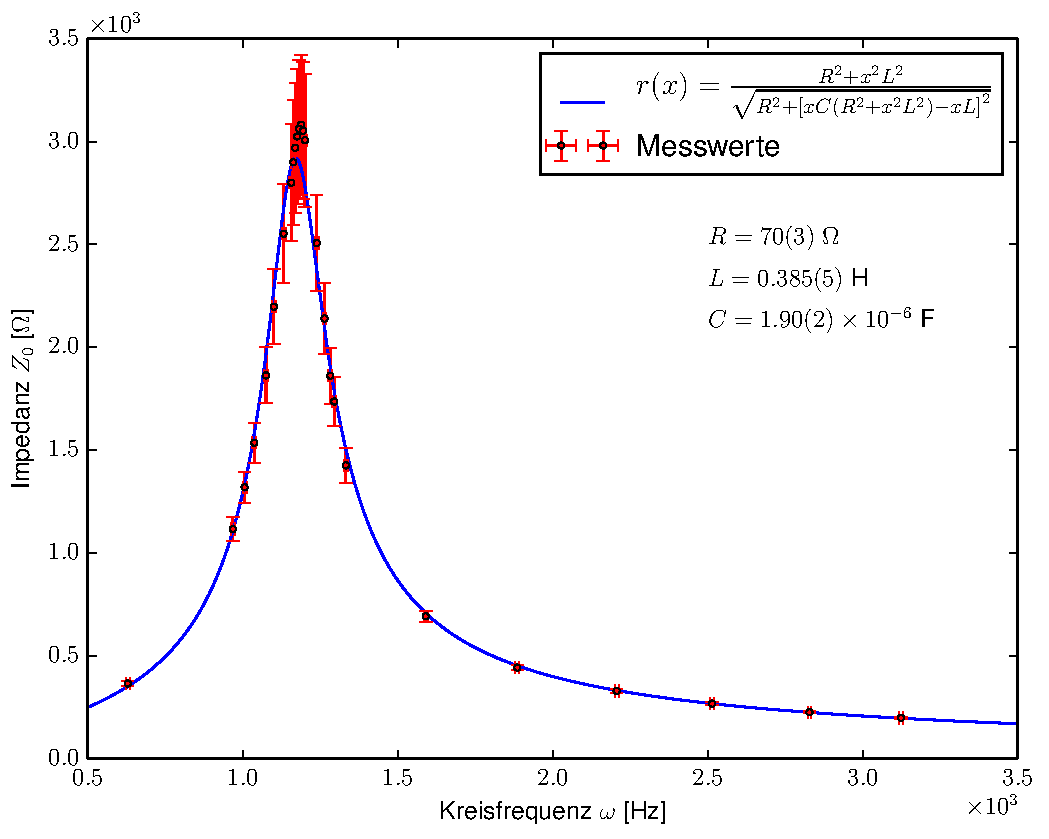
\includegraphics[width=\textwidth]{plot5.pdf}
	\caption{Auswertung des Parallelschwingkreises. Die Impedanz $Z_0$ wird über der Kreisfrequenz $\omega$ aufgetragen. Mit einem nichtlinearen Fit werden die Parameter $R$, $L$ und $C$ ermittelt. In rot sind die Messwerte mit Fehlerintervallen, in blau die Regressionskurve zu sehen.}
	\label{fig:plot5}
\end{figure}
\subsection{Zusammenfassung}
\subsubsection{\person{Ohm}scher Widerstand der Spule $R_L$}
Für den gesamten \person{Ohm}schen Widerstand im Serienschwingkreis stehen zwei Ergebnisse aus Sektionen \ref{sec:lin} und \ref{sec:serienresonanzkreis} zur Verfügung. Der gewichtete Mittelwert aus ihnen beträgt
\begin{align}
	\overline{R}&=(83.4\pm0.9)~\mrm{\Omega}.
	\label{eq:Rmittel}
\end{align}
Die Reihenschaltung besteht aus dem \person{Ohm}schen Festwiderstand $R_1$, dem Spulenwiderstand $R_L$ und dem Innenwiderstand des Amperemeters $R_i$. Mit der Maschenregel nach Sektion \ref{sec:reihepara} gilt
\begin{align}
	R=R_1+R_L+R_i\aeqiv R_L=R-R_1-R_i,
	\label{eq:Rges}
\end{align}
wobei sich der Fehler nach \person{Gauss} berechnet:
\begin{align}
	\sigma_{R_L}=\sqrt{\sigma_{R_1}^2+\sigma_{R}^2+\sigma_{R_i}^2}.
	\label{eq:sigmaRges}
\end{align}
Der Innenwiderstand des Amperemeters für die beiden verwendeten Messbereiche wurde mit einem Multimeter gemessen (Tabelle \ref{tab:widampere}).
\begin{table}[H]
	\centering
	\begin{tabular}{l|l}
		\hline
		Messbereich&Innenwiderstand\;[$\Omega$]\\\hline
		200\;mA&$1.5\pm0.5$\\
		20\;mA&$11\pm0.1$\\\hline

	\end{tabular}
	\caption{Widerstände des Amperemeters}
	\label{tab:widampere}
\end{table}
Bei der Versuchsdurchführung wurde versäumt, für jede Messreihe einen einheitlichen Messbereich zu verwenden. Als Näherung wird deshalb das arithmetische Mittel aus beiden Messbereichen verwendet:
\begin{align}
	\overline{R_i}=(7\pm0.3).
	\label{Rimittel}
\end{align}
Um beide Messbereiche gleich zu gewichten, wird der Fehler ebenfalls gemittelt.
Der \person{Ohm}sche Festwiderstand beträgt nach \cite[121]{prakti}
\begin{align}
	R_1=(10\pm1)~\Omega.
	\label{eq:Rfest}
\end{align}
Nach Gleichung \eqref{eq:Rges} erhält man für den Widerstand der Spule
\begin{align}
	R_L=(66\pm2)~\Omega.
	\label{eq:Rl}
\end{align}
Der mit dem Multimeter bestimmte Spulenwiderstand ist
\begin{align}
	R_{L,\mrm{Mess}}=(68.0\pm0.1)~\Omega.
	\label{eq:Rlmess}
\end{align}
Der aus den Messreihen bestimmte Spulenwiderstand ist somit um $3\%$ kleiner als der mit dem Multimeter gemessene Wert.
\subsubsection{Resonanzfrequenz $\omega_r$}
Aus den Sektionen \ref{sec:serienresonanzkreis} und \ref{sec:phasenverschiebung} liegen zwei Werte für die Resonanzfrequenz $\omega_r$ vor. Der gewichtete Mittelwert beträgt
\begin{align}
	\overline{\omega_r}=(1174\pm3)~\mrm{Hz}.
	\label{omegarmittel}
\end{align}
\subsubsection{Induktivität $L$}
Die erhaltenen Werte für die Induktivität $L$ stammen aus der linearen Regression aus Sektion \ref{sec:lin}, sowie aus allen drei nichtlinearen Fits. Als gewichteter Mittelwert ergibt sich
\begin{align}
	\overline{L}=(0.394\pm0.003)~\mrm{H}.
	\label{eq:Induktmittel}
\end{align}
\subsubsection{Kapazität $C$}
Für die Kapazität $C$ des Kondensators stehen zunächst die Werte aus den drei nichtlinearen Fits zur Verfügung. Alternativ ergibt sich mit Gleichung \eqref{eq:resonanz} und den zuvor errechneten Mittelwerten $\overline{\omega_r}$ und $\overline{L}$:
\begin{align}
	C_{\text{alternativ}}&=\frac{1}{\overline{L} \cdot \overline{\omega_r}^{2}}=(1.84\pm0.02)~\SI{}{\micro\farad}\\
	\sigma_{C_{\text{alternativ}}}&=\frac{1}{\overline{L}^{2} \cdot \overline{\omega_r}^{3}} \cdot \sqrt{4 \cdot \overline{L}^{2} \cdot \sigma_{\overline{\omega_r}}^{2} + \sigma_{\overline{L}}^{2} \cdot \overline{\omega_r}^{2}}.
	\label{eq:alternativ}
\end{align}
Für den gewichteten Mittelwert aus diesen vier Größen erhält man:
\begin{align}
	\overline{C}=(1.85\pm0.01)~\SI{}{\micro\farad}.
	\label{eq:cmittelfit}
\end{align}
Mit dem Multimeter wurde ein Wert von $C_{\mrm{Mess}}=(2.193\pm0.001)~\SI{}{\micro\farad}$ gemessen. Der Mittelwert aus den Auswertungen weicht um $16\%$ vom Multimeterwert ab. 
\subsubsection{Phasenverschiebung zwischen $U_{L+R}$ und $U_C$}
Nach Gleichung \eqref{eq:phase} gilt für die Phasenverschiebung zwischen $U_{L+R}$ und $U_C$:
\begin{align}
	\varphi_{\text{Theorie}}&=\operatorname{atan}{\left (\frac{\overline{L}}{\overline{R}} \cdot \overline{\omega_r} \right )}\\
	\sigma_{\varphi_{\text{Theorie}}}&=\frac{1}{\overline{L}^{2} \cdot \overline{\omega_r}^{2} + \overline{R}^{2}} \cdot \sqrt{\overline{L}^{2} \cdot \overline{R}^{2} \cdot \sigma_{\overline{\omega_r}}^{2} + \overline{L}^{2} \cdot \sigma_{\overline{R}}^{2} \cdot \overline{\omega_r}^{2} + \overline{R}^{2} \cdot \sigma_{\overline{L}}^{2} \cdot \overline{\omega_r}^{2}}.
	\label{eq:phasetheo}
\end{align}
Es ergibt sich eine Phasenverschiebung von 
\begin{align}
	\varphi_{\text{Theorie}}=(1.393 \pm 0.002)~\text{rad}.
	\label{eq:resphasetheo}
\end{align}
Der zuvor in Sektion \ref{sec:zeiger} berechnete Wert von $\varphi_{\mrm{Zeiger}}=(1.37\pm0.08)~$rad ist um 2\% kleiner als der Theoriewert. 

\section{Diskussion}
\label{sec:diskussion}

\begin{table}[H]
	\centering
	\footnotesize
	\begin{tabular}{|c|c|c|c|}
		\hline
		\person{Ohm}scher Wid.\;[$\Omega$]&Impedanz\;[H]&Resonanzfrequenz\;[Hz]&Kapazität\;[\textmu F]\\\hline\hline
		$R_{\mrm{lin}}=(76\pm18)$&$L_{\mrm{lin}}=(0.404\pm0.007)$&$\omega_{r,1}=(1175\pm3)$&$C_{\mrm{fit,1}}=(1.80\pm0.02)$\\
		$R_{\mrm{fit,1}}=(83.4\pm0.9)$&$L_{\mrm{fit,1}}=(0.403\pm0.005)$&$\omega_{r,2}=(1175\pm7)$&$C_{\mrm{fit,2}}=(1.87\pm0.03)$\\
		&$L_{\mrm{fit,2}}=(0.390\pm0.005)$&&$C_{\mrm{fit,3}}=(1.90\pm0.02)$\\
		&$L_{\mrm{fit,3}}=(0.385\pm0.005)$&&$C_{\text{alternativ}}=(1.84\pm0.02)$\\
		&&&\\
		$\overline{R}=(83.4\pm0.9)$&$\overline{L}=(0.394\pm0.003)$&$\overline{\omega_r}=(1174\pm3)$&$\overline{C}=(1.85\pm0.01)$\\
		$R_{L}=(66\pm2)$&&&\\\hline
		$R_{L,\mrm{Mess}}=(68.0\pm0.1)$&&&$C_{\mrm{Mess}}=(2.193\pm0.001)$\\\hline
	\end{tabular}
\end{table}
\begin{table}[H]
	\centering
	\begin{tabular}{|c||c|c|}
		\hline
		Phasenverschiebung [rad]&$\varphi_{\mrm{Zeiger}}=(1.37\pm0.08)$&$\varphi_{\mrm{Theorie}}=(1.393\pm0.002)$\\\hline
	\end{tabular}
	\caption{Zusammenfassung aller Ergebnisse.}
	\label{tab:ergebnisse}
\end{table}
In Tabelle \ref{tab:ergebnisse} sind alle Ergebnisse aufgeführt.
\subsection{Fehlerintervalle und relative Fehler}
Zunächst soll die Wahl der Fehlerintervalle diskutiert werden. Es ist anzumerken, dass die verwendeten Fehler für die Strom- und Spannungswerte, wie sie in Tabelle \ref{tab:messfehler} zu sehen sind, relativ großzügig gewählt wurden. Besonders bei der linearen Regression aus Sektion \ref{sec:lin} spiegeln sich die großen Fehler in Form von einem hohen relativen Fehler bei dem \person{Ohm}schen Widerstand $R_{\mrm{lin}}$ wider. Der relative Fehler beträgt hier $24\%$. Trotz der großzügigen Fehlerintervalle ist der Induktivitätswert aus der linearen Regression $R_{\mrm{lin}}$ wesentlich präziser. Hier ergibt sich ein relativer Fehler von nur $2\%$. Dies ist damit zu erklären, dass alle Messwerte sehr genau auf einer Geraden liegen. Eine Änderung der Fehlerintervalle gibt zwar eine große Freiheit beim Ordinatenabschnitt, jedoch nicht bei der Steigung.  Insgesamt fallen alle relativen Fehler unerwartet gering aus. Die mitunter präzisesten Ergebnisse sind die beiden Resonanzfrequenzen $\omega_{r,1/2}$ mit nur 0.3\% relativem Fehler. Dies liegt daran, dass während des Versuchs die Resonanzstelle sehr genau mit dem Frequenzregler abgetastet wurde und das Oszilloskop einen sehr genauen Wert angegeben hat. Die Genauigkeit bei der theoretischen Phasenverschiebung $\varphi_{\mrm{Theo}}$ mit einem relativen Fehler von nur $0.2$\% ist eine direkte Konsequenz der Genauigkeit der Frequenzen und Induktivitäten. Abgesehen von $R_{\mrm{lin}}$ sind die relativen Fehler nicht größer als $3\%$.
\subsection{Nichtlineare Fits}
Der nichtlineare Fit der gesamten Impedanz $Z_0$ aus Sektion \ref{sec:serienresonanzkreis} hat eine große Güte. Die Parameter haben alle einen niedrigen relativen Fehler und die Regressionskurve schneidet alle Fehlerintervalle. Im Gegensatz zu den etwas großen Fehlerintervallen bei der linearen Regression sehen diese hier wesentlich sinnvoller aus. Der Serienschwingkreis wirkt wie eine Art Bandpass: Bei der Resonanzstelle ist die Impedanz minimal und der Strom maximal. Die sehr geringen Fehler an der Resonanzstelle ergeben somit Sinn, da bei höheren Strömen der Innenwiderstand des Amperemeters zu geringeren Abweichungen führt. 
Der Fit der Phasenverschiebung aus Sektion \ref{sec:phasenverschiebung} ist am schwierigsten durchzuführen. Versucht man, die Theoriekurve mit allen drei Parametern $R$, $L$ und $C$ zu fitten, so versagt die Regression komplett und es ergeben sich Fehler von ca $3000\%$. Der Fit gelingt, sobald man $R$ festhält. Obwohl die relativen Fehler der Parameter niedrig sind, erkennt man deutliche Abweichungen der Regressionskurve zu den Messfehlern. Besonders bei niedrigen Frequenzen liegen die Messwerte relativ weit über der Kurve. Ein möglicher Grund hierfür ist, dass mehr Messpunkte über der Resonanzfrequenz zur Verfügung stehen als unterhalb von ihr. So wird der Fit für hohe Kreisfrequenzen genauer, büßt aber Genauigkeit bei niedrigen Kreisfrequenzen ein.
Der Fit des Parallelresonanzkreises aus Sektion \ref{sec:parakreis} verlief ähnlich gut wie der des Serienkreises. Wieder schneiden alle Vertrauensintervalle die Fitkurve und die erhaltenen Parameter haben eine hohe Präzision. Der Parallelkreis wirkt wie eine Art Sperrfilter: Ströme nahe der Resonanzfrequenz werden geschwächt, während Ströme in den restlichen Bereichen nahezu unblockiert durchgelassen werden. Im Gegensatz zum Serienkreis sind deshalb bei diesem Fit die Messwerte außerhalb der Resonanzstelle genauer. Bei der Resonanzstelle unterschätzt die Fitkurve die Messwerte ein wenig. Dennoch liegt die Kurve gut in allen Fehlerintervallen.
\subsection{Bestimmung des Spulenwiderstands $R_L$}
Bei den Werten des \person{Ohm}schen Widerstandes fällt auf, dass der gewichtete Mittelwert der gleiche ist, wie der des nichtlinearen Fits. Dies liegt an der großen Abweichung von $R_{\mrm{lin}}$. Die große Abweichung ist jedoch berechtigt, da der bestimmte Wert von $R_L$ mit nur $3\%$ Abweichung zum Multimeterwert $R_{L,\mrm{Mess}}$ sehr gut mit dem Referenzwert übereinstimmt. Es überlappen sich ebenfalls die Vertrauensintervalle dieser beiden Werte. Somit war diese Messung ein voller Erfolg.
\subsection{Bestimmung der Kapazität}
Die Bestimmung der Kapazität ist beeinflusst von der Impedanz, der Resonanzfrequenz und der nichtlinearen Fits. Wie bereits gesagt, liefern die Fits gute Werte. Die Impedanzen und Resonanzfrequenzen haben alle eine sehr hohe Präzision. Trotz der hohen Präzision und vorallem der hohen Konsistenz bei den bestimmten Kapazitätswerten, liegt der mit dem Multimeter gemessene Wert bei weitem außerhalb des Vertrauensintervalls von  $1~\sigma$. Der Mittelwert liegt ganze $16\%$ unterhalb des Multimeterwertes. Es wurde bei der Multimetermessung ein sehr geringer Fehler angenommen, jedoch ist die Abweichung zu groß, um den Fehler anzupassen. Man muss hier also von einem systematischen Fehler ausgehen. Einerseits können Kapazitätsmessungen mit Multimetern einen großen Fehler aufweisen. Andererseits kann es zu Abweichungen bei der Theorie kommen, da kein Kondensator wirklich ideal ist. Es wäre hier interessant gewesen, die Messwerte für die Impedanzen mit der Theorie zu vergleichen, aber es wurde versäumt, die Länge der Spule zu notieren. Ahand der großen Konsistenz aller anderen Messwerte, ist es sehr wahrscheinlich, dass die Kapazitätsmessung mit dem Multimeter die fehlerhafte Messung ist.
\newpage
%\nocite{*} %sorgt dafuer, dass alles ausgegeben wird
\printbibliography[heading=bibintoc]

\end{document}
